\documentclass[12pt]{report}
\usepackage[utf8]{inputenc}
\usepackage[russian]{babel}
%\usepackage[14pt]{extsizes}
\usepackage{listings}
\usepackage{graphicx}
\usepackage{amsmath,amsfonts,amssymb,amsthm,mathtools} 
\usepackage{pgfplots}
\usepackage{filecontents}
\usepackage{indentfirst}
\usepackage{eucal}
\usepackage{float} 
\usepackage{amsmath}
\usepackage{enumitem}
\usepackage[justification=centering]{caption} 
\usepackage{tikz}

\usepackage{pgfplots}

\pgfplotsset{compat=newest}

\frenchspacing

\usepackage{indentfirst} % Красная строка


%\usetikzlibrary{datavisualization}
%\usetikzlibrary{datavisualization.formats.functions}

\usepackage{amsmath}


% Для листинга кода:
\lstset{ %
language=C++,                 % выбор языка для подсветки (здесь это С)
basicstyle=\small\sffamily, % размер и начертание шрифта для подсветки кода
numbers=left,               % где поставить нумерацию строк (слева\справа)
numberstyle=\tiny,           % размер шрифта для номеров строк
stepnumber=1,                   % размер шага между двумя номерами строк
numbersep=5pt,                % как далеко отстоят номера строк от подсвечиваемого кода
showspaces=false,            % показывать или нет пробелы специальными отступами
showstringspaces=false,      % показывать или нет пробелы в строках
showtabs=false,             % показывать или нет табуляцию в строках
frame=single,              % рисовать рамку вокруг кода
tabsize=2,                 % размер табуляции по умолчанию равен 2 пробелам
captionpos=t,              % позиция заголовка вверху [t] или внизу [b] 
breaklines=true,           % автоматически переносить строки (да\нет)
breakatwhitespace=false, % переносить строки только если есть пробел
escapeinside={\#*}{*)},   % если нужно добавить комментарии в коде
singlelinecheck=false,
}

\usepackage[left=2cm,right=2cm, top=2cm,bottom=2cm,bindingoffset=0cm]{geometry}
% Для измененных титулов глав:
\usepackage{titlesec, blindtext, color} % подключаем нужные пакеты
\definecolor{gray75}{gray}{0.75} % определяем цвет
\newcommand{\hsp}{\hspace{20pt}} % длина линии в 20pt
% titleformat определяет стиль
\titleformat{\chapter}[hang]{\Huge\bfseries}{\thechapter\hsp\textcolor{gray75}{|}\hsp}{0pt}{\Huge\bfseries}
\addto\captionsrussian{\renewcommand{\contentsname}{Содержание}}
\captionsetup{justification=raggedright,singlelinecheck=false}

% plot
\usepackage{pgfplots}
\usepackage{filecontents}
\usetikzlibrary{datavisualization}
\usetikzlibrary{datavisualization.formats.functions}

\begin{document}
%\def\chaptername{} % убирает "Глава"
\thispagestyle{empty}
\begin{titlepage}
	\noindent \begin{minipage}{0.15\textwidth}
	
\includegraphics[width=\linewidth]{b_logo}
	\end{minipage}
	\noindent\begin{minipage}{0.9\textwidth}\centering
		\textbf{Министерство науки и высшего образования Российской Федерации}\\
		\textbf{Федеральное государственное бюджетное образовательное учреждение высшего образования}\\
		\textbf{~~~«Московский государственный технический университет имени Н.Э.~Баумана}\\
		\textbf{(национальный исследовательский университет)»}\\
		\textbf{(МГТУ им. Н.Э.~Баумана)}
	\end{minipage}
	
	\noindent\rule{18cm}{3pt}
	\newline\newline
	\noindent ФАКУЛЬТЕТ $\underline{\text{«Информатика и системы управления»}}$ \newline\newline
	\noindent КАФЕДРА $\underline{\text{«Программное обеспечение ЭВМ и информационные технологии»}}$\newline\newline\newline\newline\newline
	
	
	\begin{center}
		\noindent\begin{minipage}{1.3\textwidth}\centering
			\Large\textbf{  Отчёт по лабораторной работе №5}\newline
			\textbf{по дисциплине "Анализ алгоритмов"}\newline\newline
		\end{minipage}
	\end{center}
	
	\noindent\textbf{Тема} $\underline{\text{Конвейерные вычисления}}$\newline\newline
	\noindent\textbf{Студент} $\underline{\text{Михаил Коротыч}}$\newline\newline
	\noindent\textbf{Группа} $\underline{\text{ИУ7-55Б}}$\newline\newline
	\noindent\textbf{Преподаватели} $\underline{\text{Волкова Л. Л., Строганов Ю. В.}}$\newline\newline\newline
	
	\begin{center}
		\vfill
		Москва~---~\the\year
		~г.
	\end{center}
\end{titlepage}

\tableofcontents

\newpage
\chapter*{Введение}
\addcontentsline{toc}{chapter}{Введение}

При обработке данных могут возникать ситуации, когда один набор данных необходимо обработать последовательно несколькими алгоритмами. В таком случае удобно использовать конвейерную обработку данных, что позволяет на каждой следующей <<линии>> конвейера использовать данные, полученные с предыдущего этапа. 
Помимо линейной конвейерной обработки данных, существуют параллельная конвейерная обработка данных. При таком подходе все линии работают с меньшим времени простоя, так как могут обрабатывать задачи независимо от других линий.

Целью данной лабораторной работы является изучение и реализация параллельной и линейной реализации конвейерной обработки данных. В рамках выполнения работы необходимо решить следующие задачи:

\begin{itemize}
	\item изучить конвейерную обработку данных;
	\item реализовать систему конвейерных вычислений с количеством линий не меньше трёх;
	\item сравнить параллельную и линейную реализацию конвейерных вычислений;
	\item сделать выводы на основе проделанной работы.
\end{itemize}

\chapter{Аналитическая часть}

В данном разделе представленные теоретические сведения о рассматриваемых алгоритмах.

\section{Конвейерная обработка данных}

Конвейер - система поточного производства. В терминах программирования ленты конвейера представлены функциями, выполняющими над неким набором данных операции и передающие их на следующую ленту конвейера. Моделирование конвейерной обработки хорошо сочетается с технологией многопоточного программирования - под каждую ленту конвейера выделяется отдельный поток, все потоки работают в асинхронном режиме.

\section{Описание задачи}

В качестве алгоритма, реализованного для распределения на конвейере, был выбран процес сборки автомобиля, состоящий из трёх этапов:

\begin{itemize}
	\item сборка движка (возведение числа в степень);
	\item сборка корпуса (проверка числа на простоту);
	\item сборка колёс (вычисление числа Фибоначчи).
\end{itemize}

\section{Вывод}
Ввод в программе не предусматривается. Результат представляет собой таблицу, в которой представлены количество задач, конвейеры и общее время работы в миллисекундах. К программе предъявляется ряд требований:

\begin{itemize}
	\item на вход алгоритму подаётся количество задач (количество машин, которые нужно собрать);
	\item на выходе - время, затраченное на обработку заявок;
	\item в процессе обрабатывания задач необходимо фиксировать время прихода и ухода заявки с линии.
\end{itemize}

В разделе были рассмотрены особенности построения конвейерных вычислений, описание решаемой задачи.

\chapter{Конструкторская часть}

В данном разделе представлены схемы рассматриваемых алгоритмов.

\section{Разработка алгоритмов}

На рисунке 2.1 приведена схема организации конвейерных вычислений.

\begin{figure}[h]
	\centering
	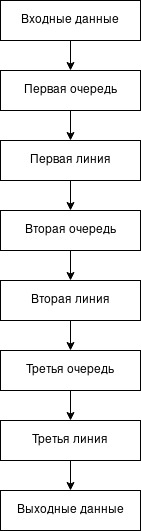
\includegraphics[scale=0.6]{scheme_lab05.jpg}
	\caption{Схема организации конвейерных вычислений.}
	\label{fig:mpr}
\end{figure}

\section{Использованные структуры данных}
Для задачи по сборке движка, корпуса и колёс были созданы классы \texttt{Engine}, \texttt{Carcass} и \texttt{Wheels} с основными характеристиками соответствующих механизмов. Класс \texttt{Car} является централизованным классом, который содержит экземпляры всех трёх остальных классов. Для логирования был создан класс \texttt{Logger}.  Он содержит метод, отвечающий за вывод данных в таблицу.

\section{Вывод}
На основе теоретических данных, полученных из аналитического раздела, была построена схема алгоритма конвейерных вычислений.

\chapter{Технологическая часть}

В данном разделе приведены средства реализации и листинги кода.

\section{Средства реализации}

Для реализации ПО я выбрал язык программирования С++ \cite{C++}. Данный выбор обусловлен не только моим опытом разработки программ на этом языке, но также и моим желанием расширить свои знания в области применения данного языка программирования.

\section{Реализация алгоритмов}

В листингах 3.1 и 3.2 приведены реализации конвейерных вычислений (класс \texttt{Cloveyor}), реализация сборки машины (класс \texttt{Car}) и реализация класса отвечающего за логирование (класс \texttt{Logger}). На рисунках 2.2-2.5 представлены интерфейс созданных классов.

\begin{figure}
	\centering
	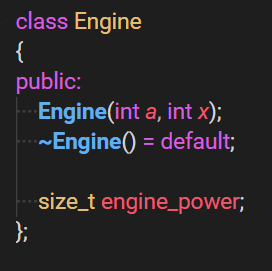
\includegraphics{Engine.PNG}
	\caption{Скриншот класса.}
	\label{fig:mpr}
\end{figure}

\begin{figure}
	\centering
	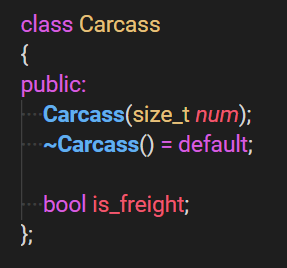
\includegraphics{Carcass.PNG}
	\caption{Скриншот класса.}
	\label{fig:mpr}
\end{figure}

\begin{figure}
	\centering
	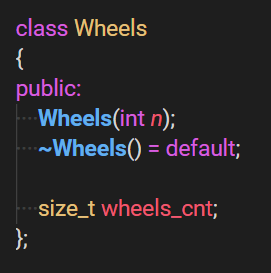
\includegraphics{Wheels.PNG}
	\caption{Скриншот класса.}
	\label{fig:mpr}
\end{figure}

\begin{figure}
	\centering
	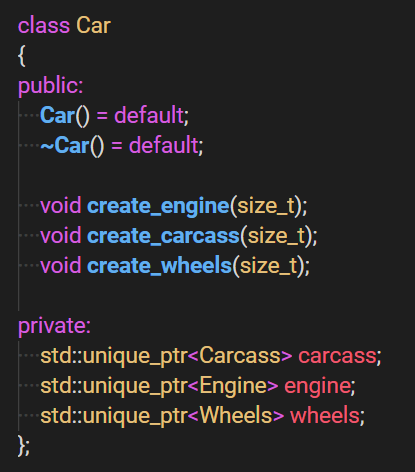
\includegraphics{Car.PNG}
	\caption{Скриншот класса.}
	\label{fig:mpr}
\end{figure}

\newpage
\begin{lstlisting}[label=some-code,caption=Реализация класса конвейера, language=C++]
#include <thread>
#include <queue>

#include "car.h"

#define THRD_CNT 3

class Conveyor
{
public:
	Conveyor() = default;
	~Conveyor() = default;
	
	void run(size_t cars_cnt);
	
	void create_engine();
	void create_carcass();
	void create_wheels();
	
private:
	std::thread threads[THRD_CNT];
	std::vector<std::shared_ptr<Car>> cars;
	
	std::queue<std::shared_ptr<Car>> q1;
	std::queue<std::shared_ptr<Car>> q2;
	std::queue<std::shared_ptr<Car>> q3;
};

void Conveyor::run_parallel(size_t cars_cnt)
{
	for (size_t i = 0; i < cars_cnt; ++i)
	{
		std::shared_ptr<Car> new_car(new Car);
		cars.push_back(new_car);
		q1.push(new_car);
	}
	
	this->threads[0] = std::thread(&Conveyor::create_carcass, this);
	this->threads[1] = std::thread(&Conveyor::create_engine, this);
	this->threads[2] = std::thread(&Conveyor::create_wheels, this);
	
	for (int i = 0; i < THRD_CNT; ++i)
		this->threads[i].join();
}

void Conveyor::run_linear(size_t cars_cnt) 
{
	for (size_t i = 0; i < cars_cnt; ++i)
	{
		std::shared_ptr<Car> new_car(new Car);
		cars.push_back(new_car);
		q1.push(new_car);
	}
	
	for (size_t i = 0; i < cars_cnt; ++i) 
	{
		std::shared_ptr<Car> car = q1.front();
		car->create_carcass(i + 1);
		q2.push(car);
		q1.pop();
		
		car = q2.front();
		car->create_engine(i + 1);
		q3.push(car);
		q2.pop();
		
		car = q3.front();
		car->create_wheels(i + 1);
		q3.pop();
	}
}

void Conveyor::create_carcass()
{
	size_t task_num = 0;
	
	while (!this->q1.empty())
	{
		std::shared_ptr<Car> car = q1.front();
		car->create_carcass(++task_num);
		
		q2.push(car);
		q1.pop();
	}
}

void Conveyor::create_engine()
{
	size_t task_num = 0;
	
	do
	{
		if (!this->q2.empty())
		{
			std::shared_ptr<Car> car = q2.front();
			car->create_engine(++task_num);
	
			q3.push(car);
			q2.pop();
		}
	} while (!q1.empty() || !q2.empty());
}

void Conveyor::create_wheels()
{
	size_t task_num = 0;
	
	do
	{
		if (!this->q3.empty())
		{
			std::shared_ptr<Car> car = q3.front();
			car->create_wheels(++task_num);
			q3.pop();
		}
	} while (!q1.empty() || !q2.empty() || !q3.empty());
}
\end{lstlisting}

\begin{lstlisting}[label=some-code,caption=Реализация класса сборки машины, language=C++]
#include <memory>
#include <cmath>

#include "logger.h"

class Carcass
{
public:
	Carcass(size_t num);
	~Carcass() = default;
	
	bool is_freight;
};

class Engine
{
public:
	Engine(int a, int x);
	~Engine() = default;
	
	size_t engine_power;
};

class Wheels
{
public:
	Wheels(int n);
	~Wheels() = default;
	
	size_t wheels_cnt;
};

class Car
{
public:
	Car() = default;
	~Car() = default;
	
	void create_engine(size_t);
	void create_carcass(size_t);
	void create_wheels(size_t);
	
private:
	std::unique_ptr<Carcass> carcass;
	std::unique_ptr<Engine> engine;
	std::unique_ptr<Wheels> wheels;
};

Carcass::Carcass(size_t num)
{
	this->is_freight = false;
	
	for (size_t i = 2; i <= sqrt(num); ++i)
		if (!(num % i))
			return;

	this->is_freight = true;
}

Engine::Engine(int a, int x)
{    
	this->engine_power = a;
	
	for (int i = 0; i < x; i++)
		this->engine_power *= a;
}

Wheels::Wheels(int n)
{
	size_t f1 = 1, f2 = 1;
	this->wheels_cnt = f1;
	
	for (int i = 2; i < n; ++i)
	{
		this->wheels_cnt = f1 + f2;
		f1 = f2;
		f2 = this->wheels_cnt;
	}
}

void Car::create_engine(size_t task_num)
{
	Logger::log_current_event(task_num, "Part 2 | Start");
	
	if (this->carcass->is_freight) 
		this->engine = std::unique_ptr<Engine>(new Engine(10, 150000));
	else
		this->engine = std::unique_ptr<Engine>(new Engine(5,  150000));

	Logger::log_current_event(task_num, "Part 2 | End  ");
}

void Car::create_carcass(size_t task_num)
{
	Logger::log_current_event(task_num, "Part 1 | Start");
	this->carcass = std::unique_ptr<Carcass>(new Carcass(27644437));
	Logger::log_current_event(task_num, "Part 1 | End  ");
}

void Car::create\_wheels(size\_t task\_num)
{
	Logger::log_current_event(task_num, "Part 3 | Start");
	this->wheels = std::unique_ptr<Wheels>(new Wheels(this->engine->engine\_power));
	Logger::log_current_event(task_num, "Part 3 | End  ");
}
\end{lstlisting}

\begin{lstlisting}[label=some-code,caption=Реализация класса логирования, language=C++]
#include <iostream>
#include <chrono>

using namespace std::chrono;

class Logger 
{
public:
	Logger() = default;
	~Logger() = default;
	
	static void log_current_event(size_t task_num, const char *const event);
}

void Logger::log_current_event(size_t task_num, const char *const event) 
{
	system_clock::time_point now = system_clock::now();
	system_clock::duration tp = now.time_since_epoch();
	
	tp -= duration_cast<seconds>(tp);
	
	time_t tt = system_clock::to_time_t(now);
	tm t = *gmtime(&tt);
	
	std::printf
	(
		"Task #%lu | %s | %02u:%02u:%02u.%3u\n", 
		task_num,
		event, 
		t.tm_hour, 
		t.tm_min, 
		t.tm_sec, 
		static_cast<unsigned>(tp / milliseconds(1))
	);
}
\end{lstlisting}

%\section{Тестовые данные}

\section{Вывод}

В данном разделе была разработана и рассмотрена реализация конвейерных вычислений.

\chapter{Исследовательская часть}

В данном разделе приведен анализ характеристик разработанного ПО  и примеры работы ПО.

\section{Пример работы программы}

\begin{figure}
	\centering
	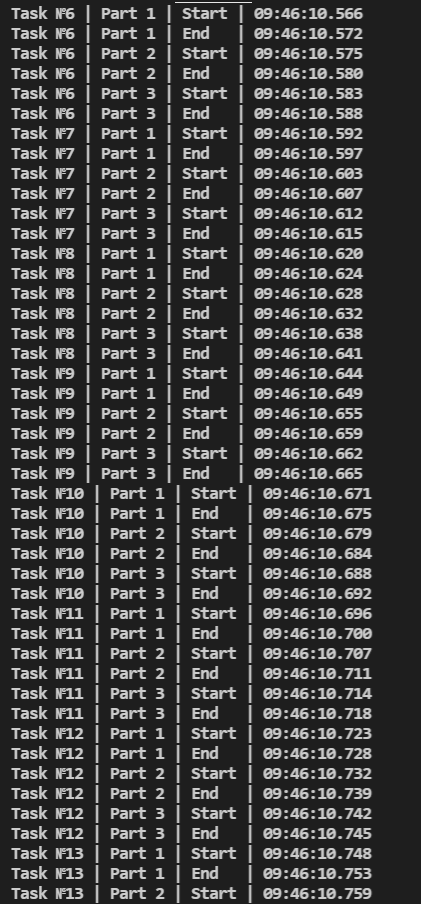
\includegraphics[scale=0.8]{prog_ex.png}
	\caption{Пример работы программы (параллельная обработка)}
	\label{fig:conveyor}
\end{figure}

\section{Технические характеристики}

Ниже приведены технические характеристики устройства, на котором было проведено тестирование ПО:

\begin{itemize}
	\item операционная система: Windows 10 21H2;
	\item оперативная память: 8 ГБ;
	\item процессор: Intel(R) Core(TM) i7-8550U CPU @ 1.80GHz   1.99 GHz.
\cite{i5}.

\end{itemize}

\section{Время выполнения алгоритмов}

Время выполнения алгоритма замерялось с помощью применения технологии профайлинга \cite{profiling}. Данный инструмент даёт детальное описание количество вызовов и количества времени CPU, затраченного на выполнение каждой функции.

В таблице \ref{tab01} приведено сравнение времени выполнения параллельной обработки данных (сборка машины), в зависимости от количества входных задач (количества машин). Линия №1 - сборка каркасов автомобилей (проверка числа на простоту), линия №2 - сборка двигателей автомобилей (возведение числа в степень), линия №3 - сборка колёс автомобилей (вычисление числа Фибоначчи). Время указано в секундах.

\begin{table} [h!]
	\caption{Таблица времени выполнения параллельной обработки данных, время в секундах}
	\label{tab01}
	\begin{center}
		\begin{tabular}{|c c c c|} 
		 	\hline
			№ линии & Task M & Начальное время & Конечное время\\
		 	\hline
		 	1 & 1 & 19:18:41.210 & 19:18:41.220\\
		 	\hline
		 	1 & 2 & 19:18:41.224 & 19:18:41.228\\
		 	\hline
		 	1 & 3 & 12:43:08.020 & 12:43:08.224\\
		 	\hline
			2 & 1 & 19:18:41.224 & 19:18:41.232\\
			\hline
			2 & 2 & 19:18:41.241 & 19:18:41.252\\
			\hline
			2 & 3 & 19:18:41.264 & 19:18:41.275\\
			\hline
			3 & 1 & 19:18:41.241 & 19:18:41.248\\
			\hline
			3 & 2 & 19:18:41.264 & 19:18:41.267\\
			\hline
			3 & 3 & 19:18:41.290 & 19:18:41.294\\
			\hline
			4 & 1 & 19:18:41.260 & 19:18:41.279\\
			\hline
			4 & 2 & 19:18:41.297 & 19:18:41.320\\
			\hline
			4 & 3 & 19:18:41.330 & 19:18:41.339\\
			\hline
		\end{tabular}
	\end{center}
\end{table}

На рисунке \ref{plt:linear-vs-parallel} представлен график зависимости времени от количества задач для линейной и параллельной обработки конвейера.

\begin{figure}[H]
	\centering
	\begin{tikzpicture}
	\begin{axis}[
	axis lines=left,
	xlabel=Размерность матрицы,
	ylabel={Время, мс},
	legend pos=north west,
	ymajorgrids=true
	]
	\addplot table[x=size,y=Linear,col sep=comma]{data/linear.csv};
	\addplot table[x=size,y=Parallel,col sep=comma]{data/parallel.csv};
	\legend{Линейный, Параллельный}
	\end{axis}
	\end{tikzpicture}
	\captionsetup{justification=centering}
	\caption{Зависимость времени работы реализации конвейеров от количества задач}
	\label{plt:linear-vs-parallel}
\end{figure}

\section{Вывод}

В данном разделе приведены время исполнения параллельного алгоритма и его сравнение с линейной реализацией конвейера. Как видно из таблицы \ref{tab01}, вторая линия, то есть сборка двигателей (возведение числа в степень) занимает в среднем 70\% времени от выполнения всей программы. Линия №3 в среднем работает быстрее чем линия №1.

Параллельная реализация конвейерной обработки выигрывает по времени исполнения у линейной реализации. Как видно из рисунка \ref{plt:linear-vs-parallel}, линейная реализация работает в 3 раза медленнее при 200 задачах.

\chapter*{Заключение}
\addcontentsline{toc}{chapter}{Заключение}

В рамках данной лабораторной работы лабораторной работы была достигнута её цель: изучена параллельная и линейная реализация конвейерной обработки данных. Также выполнены следующие задачи:

\begin{itemize}
	\item изучена конвейерная обработка данных;
	\item реализована система конвейерных вычислений с количеством линий не меньше трёх;
	\item сравнены параллельные и линейные реализации конвейерных вычислений;
	\item сделаны выводы на основе проделанной работы;
\end{itemize}

Параллельные конвейерные вычисления позволяют организовать непрерывную обработку данных, что позволяет выиграть время в задачах, где требуется обработка больших объёмов данных за малый промежуток времени.

\addcontentsline{toc}{chapter}{Список литература}
\bibliographystyle{utf8gost705u}  % стилевой файл для оформления по ГОСТу
\bibliography{51-biblio}          % имя библиографической базы (bib-файла)
[4] Windows 10. Режим доступа: https://www.microsoft.com/ru-ru/windows/get-windows-10. Дата обращения: 21.11.2021

[5] Вычислительные конвейеры. Режим доступа: http://kspt.icc.spbstu.ru/media/files/2018/kuzmin/Chapter5.pdf. Дата обращения 21.11.2021
\end{document}